\chapter{Key tools--INLA and SPDE}

\section{Random fields in practice -- approximating a continuous structure}

\subsection{Approximation by a regular grid}
\subsection{Approximation by a triangulation}

\section{Random fields in practice -- computational challenges}
There are computational challenges with random fields.

\subsection{Why are random fields hard to fit?}

\section{INLA}


Clearly, spatial point patterns are a data structure that lives in \textbf{continuous space}. However, when fitting the models we have discussed so far we have been using a spatially discrete gridding approach, where the point pattern is approximated by a grid of counts and the model is fitted as a \texttt{glm} type model with a Gauss Markov random field accounting for spatial (and temporal) autocorrelation. 

In this chapter, we point out a key disadvantage of this approach along with the benefits we get from using it -- and provide an outlook on a new method that has recently been developed by Lindgren et al.\ 2011 and does not have this key disadvantage. This method -- referred to as the \textbf{SPDE approach}\footnote{SPDE stands for ``stochastic partial differential equation". We explain why SPDEs are relevant later in the chapter. For now, the reader should not worry about the method's name too much.} --  uses a spatially continuous representation of the point pattern and is more flexible than the gridding approach in many ways while still being computationally efficient. Indeed, we will see that in many realistic cases the approach is even more  efficient, precisely due to its flexibility. And what is more, it can still be used within the \texttt{R-INLA} framework! 

In the context of this book we can currently only provide a taster of this new methodology as it is still evolving. This is particularly true for the code and the associated \texttt{R}-functions currently implemented in \texttt{R-INLA} for these methods. However, we will show examples to provide some background and outlook onto what is coming.  It is likely that the code used in these examples will change or that in the future some of this can be coded more elegantly. Updates on the software may be found on the \texttt{R-INLA} webpage.  In particular, a tutorial on the SPDE approach written by Elias Krainski and Finn Lindgren is available on these webpages, providing up-to-date information on the software.

\section{ Why gridding?}
Throughout this book the initial step in any of the analyses we have discussed consisted of gridding the data. We know that INLA operates on gridded data -- lets recall briefly why \textit{exactly}  this is the case. 
\subsection{Advantages and disadvantages of the gridding approach}
Gridding spatial data such as a point pattern for model fitting in general -- and in particular in the approach we have taken here -- has a number of benefits.  For one thing, it is rather intuitive. If you are using point pattern data to understand ``where things are" admitting a grid on your observation window  and counting how many objects you find in each of the grid cells sounds like a sensible way forward and  is clearly easy to understand.  
   
In addition, when working through all the different models we have seen so far, we have certainly noticed that using the gridding approach is also very useful.  It makes the fitting of even rather complex models computationally feasible since we can use Gauss Markov random fields to represent spatial structures. These have sparse matrices that  represent the spatial correlation structure and computation with these is very  efficient.
A further benefit of the gridding approach is that the grid we have been using is a \textbf{regular grid}. In this way we make sure that the models are resolution and distance consistent. 

However, the gridding approach also has (at least) one big \textbf{disadvantage}. Through gridding the data
we lose a lot of information -- we are moving several points to some representative location of a grid cell forgetting about the real location of the individual points. 
Clearly, this loss of information gets smaller with a finer the grid. However, the finer the grid the less computationally efficient we get... 

\subsection{Double-role of the grid}
Put differently, the above means that the grid has two different roles: 
\begin{enumerate}
\item it approximates the spatially continuous (Gaussian) random field by a discrete GM random field and
\item it approximates the locations of the points.
\end{enumerate}
While the first role is sensible as it is one of the key ingredients that INLA relies on to improve computational efficiency (see Chapter 2), the second role leads to a loss of information. While we have point pattern data that are given in spatially continuous space, we bin these data, forgetting about the exact location of the points. 
Hence, in an ideal world we would like to have an approach that has all the benefits of the gridding approach but without the disadvantage of loosing some of the information we have. So our wish-list for the perfect approach would require it to 
\begin{itemize}
\item be computationally efficient
\item be resolution consistent and make sense on non-regular lattices, scaling distances appropriately
\item be easy to use
\item be a spatially continuous representation of point locations without a loss of information
\item avoid the no double-role of a grid, i.e.\ use the grid only approximate the random field.
\end{itemize}

The good news is -- such an approach exists, the SPDE approach. And what is more -- this approach is more flexible than the gridding approach and allows us to do things that we cannot do with the gridding approach. The downside is that some of the maths behind the approach is very technical (no wonder that it has only been developed very recently...) -- but there is also some good news to be told. The new approach can be implemented in \texttt{R-INLA} and the user can ignore most of the technical details.  This chapter introduces the SPDE approach trying to avoid most of the technical detail. 

We will initially explain how it represents space -- and hence spatial point patterns -- in a spatially continuous way while still approximating the random field.

\section{The SPDE approach in a nutshell}
\subsection{Spatially continuous representation -- the mesh}
In order to obtain a spatially continuous representation of the log Gaussian Cox process we use an approximation of continuous space that we will refer to as the ``mesh". This is a triangulation of the space, based on a regular triangulation  or a triangulation that is constructed so that model fitting is computationally efficient.  We will see in Section \ref{spdeexamples} that it can be more computationally efficient to use a non-regular triangulation -- for example in cases where data could not be observed in some part of the observation window.  

The triangulation as implemented  in \texttt{R-INLA} (and as described in Lindgren et al.\ 2011)  is based on an initial \textbf{Delaunay triangulation} \footnote{A Delaunay triangulation of a given set of points is the triangulation that maximises the smallest angle among all the triangle angles.} of an initial set of points. These points  may be some or all of the data points, but this is not required or even always desirable as initial points that are strongly clustered can cause numerical problems. Further points are then added successively in additional locations in the observation window to improve the following two criteria until they are fulfilled. These are the maximum edge length and the minimum angle, respectively:
\begin{enumerate}
\item \texttt{max.edge} = the longest allowed length of any triangle edge,
\item \texttt{min.angle} = the smallest allowed angle in any triangle,
\end{enumerate}
and they are chosen by the user. The maximum edge length is relevant since it determines the minimum spatial scale at which structures are relevant and should typically be chosen to be at least smaller than the spatial
correlation range. The second criterion favours near-equilateral triangles over ``skinny" triangles. This is useful if triangles of different sizes are used as it facilitates the transition from large to small triangles and vice versa. We will come back to the choice of these values in the examples in Section \ref{spdeexamples}. Figure \ref{surface_mesh} shows an example of a regular mesh.
\begin{figure}[t]
  \centering
   \mbox{
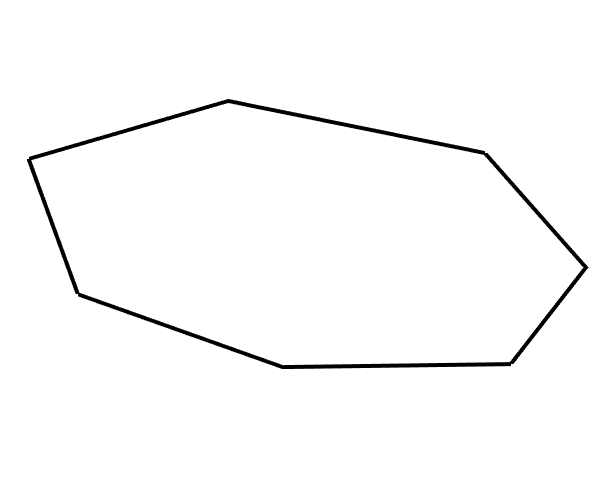
\includegraphics[width= 0.4\textwidth, angle= 0]{no_mesh.png}

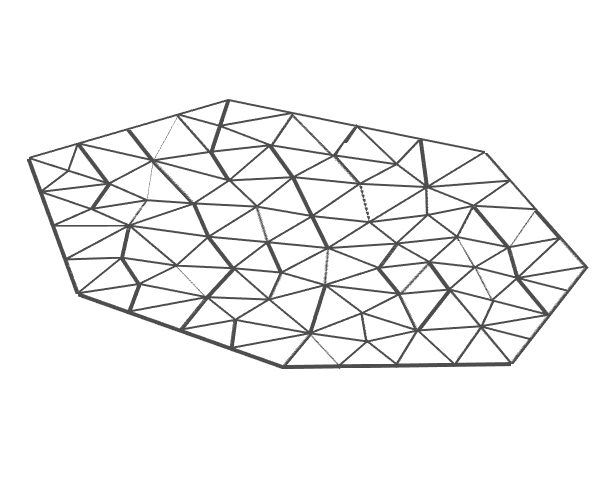
\includegraphics[width= 0.4\textwidth, angle= 0]{mesh_only.png}
}
\caption{ A regular mesh approximating an observation window. \texttt{Probably also plot an irregular grid?} \label{surface_mesh}}
\end{figure}

Based on the triangulation, i.e.\ the mesh, we now construct an approximation to the smooth, spatially continuous surface by taking true values from the surface in a set of well-designed points and interpolate the surface by \textbf{piecewise linear functions}.  This is very similar to approximating a curve by a piece-wise linear function (see Figure ???). These are functions that consist of bits of lines that take on exact values and are are glued together in ``exact" points. However, recall that we consider the two-dimensional case here. This means this we are approximating a surface by bits of flat planes. These also take on exact values in some points but are glued together along the edges of the mesh.  
%These functions are defined over out triangular mesh, which gives us more geometric flexibility than a traditional grid-based %method. 

The most intuitive way to think about this is as trying to approximate smooth surface by  a piece of crumpled -- and unfolded -- paper. A realisation from the spatially continuous Gaussian field that we would like to approximate is similar to a piece of fabric and we approximate this by a (very nicely and cleverly)  crumbled paper. Figure \ref{surface_reconstruction} shows a sketch of what this looks like.
\begin{figure}[t]
  \centering
   \mbox{
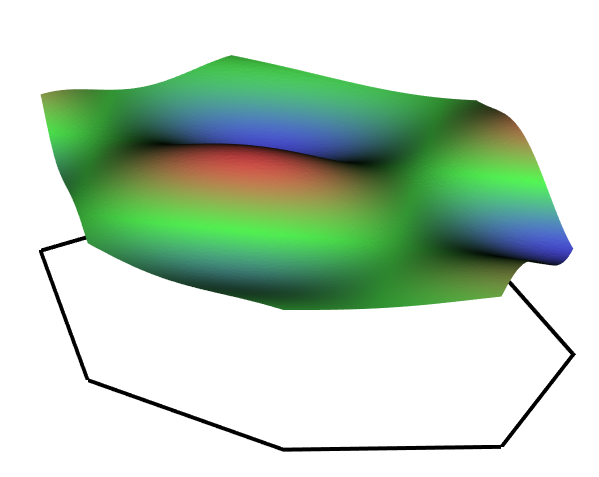
\includegraphics[width= 0.4\textwidth, angle= 0]{fcn1.png}

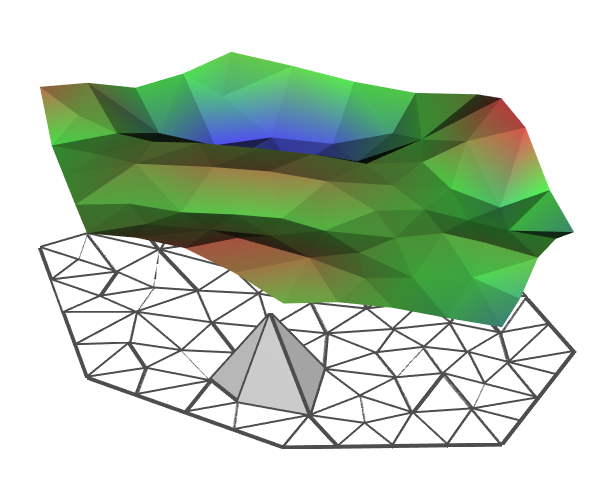
\includegraphics[width= 0.4\textwidth, angle= 0]{fcn2.png}
}
\caption{An example of a piecewise linear approximation to a surface.  The grey pyramid is a representative basis function. \label{surface_reconstruction}}
\end{figure}

\subsection{Mat\'{e}rn fields on the mesh  -- motivation}
Through the triangulation and the linear functions we now have a continuous representation of the continuous surface -- but this is just a representation, not a stochastic model that governs the surface. In other words, what we need now is a structure that is similar to the random walk and  Mat\'{e}rn random field models in Chapter 3 -- but not operating on the grid but on the triangulation.

This structure is a specific subset of the Mat\'{e}rn random fields (technical details of the subset  are given in Section \ref{matern_tech}).  These stochastic fields have parameters that govern the strength and range of spatial autocorrelations. However, unlike in the gridding approach where we approximate a (spatially continuous) Gaussian field by Gauss Markov random field without explicitly linking the GMRV to a specific GF we now have an explicit link.  This link is constructed by interpreting the Gaussian field as the solution to a stochastic differential equation and then approximating the SPDE by a GMRV.
 
This implies that the parameters of the Gaussian field translate into the parameters of the SPDE and model interpretation may be done on the basis of the SPDE -- potentially facilitating model construction and intuition.
Further, this also comes with the benefit that we do not have define the GF directly (which can be hard!) but can construct more complex spatial fields through the SPDE (see Section \ref{benefit}). It also implies that, like the Gauss Markov random fields we have seen above, the new GMRF also has a local dependence structure  with a sparse precision matrix making the approach computationally efficient.

\subsection{Mat\'{e}rn fields on the mesh  -- technical details}\label{matern_tech}

Technically speaking, the subset of the Mat\'{e}rn random fields we mention above are zero-mean Gaussian stationary, isotropic random fields with covariance function $$
c(h) = \frac{\sigma^2}{\Gamma(\nu) 2^{\nu-1}}(\kappa h)^\nu K_\nu(\kappa h), \qquad h \geq 0,
$$ where $K_\nu(\cdot)$ is the modified Bessel function of the second kind, $\nu>0$ is the smoothing parameter, $\kappa >0$ is the range parameter, and $\sigma^2$ is the variance. The subset  of Mat\'{e}rn random fields with efficient piecewise linear representations occur when $\nu + d/2$ is an integer, where $d$ is the dimension of the space.

When  $\nu + d/2$ is an integer, a computationally efficient piecewise linear representation can be constructed by using a different representation of the Mat\'{e}rn field $x(s)$, namely as the stationary solution to the stochastic partial differential equation (SPDE) \begin{equation} \label{SPDE}
(\kappa^2 - \Delta)^{\alpha/2} x(s) = W(s),
\end{equation} where $\alpha= \nu - d/2$ is an integer, $\Delta = \sum_{i=1}^d \frac{\partial^2 }{\partial s_i^2}$ is the Laplacian operator and $W(s)$ is spatial white noise.  This representation had first been constructed by \citet{art246,art455} while proving (among other things) that the classical second order conditional autoregression (CAR(2)) model limits to a Mat\'{e}rn field with $\nu = 1$.

\subsection{Further benefits of the SPDE approach}\label{benefit}
We have set out saying that the SPDE approach is promising and useful as it does not approximate the locations of the points. However, this is not the only benefit we get from using this approach. It also gives use much more flexibility when constructing models. Without going into too much technical detail -- this is mainly because the SPDE in equation \ref{SPDE} can be generalised to account for more complex models. In particular, these can be models that account for non-stationarity in the data such that the spatial autocorrelation varies in space or follows some directionality. Similarly, it also allows us to build models on domains that are more complex than a simple rectangle or polygon, including a sphere (the earth!) or domains with holes. The following will illustrate a few examples of complex random fields that may be constructed with the SPDE approach.

\subsubsection{Spatial fields on complex domains}
In practice, the observation area in a study is no always a nice rectangle or well-behaved polygon -- especially in studies of animals for whom a large observation area has to be considered. This tends to imply that the observation area contains ``holes", i.e.\ sub-areas in which the animals are unlikely to be observed.  For example, if data on aquatic animals (say whales) are of interest the observation area might contain islands where the animals are unlikely to be observed and which are perceived as barriers by the animals.  This implies that we do not want to model on these islands, and also that we do not want to consider distances across the islands. Figure \ref{complex} shows an example of a spatial field in a complex domain.
\begin{figure}[t]
  \centering
   \mbox{
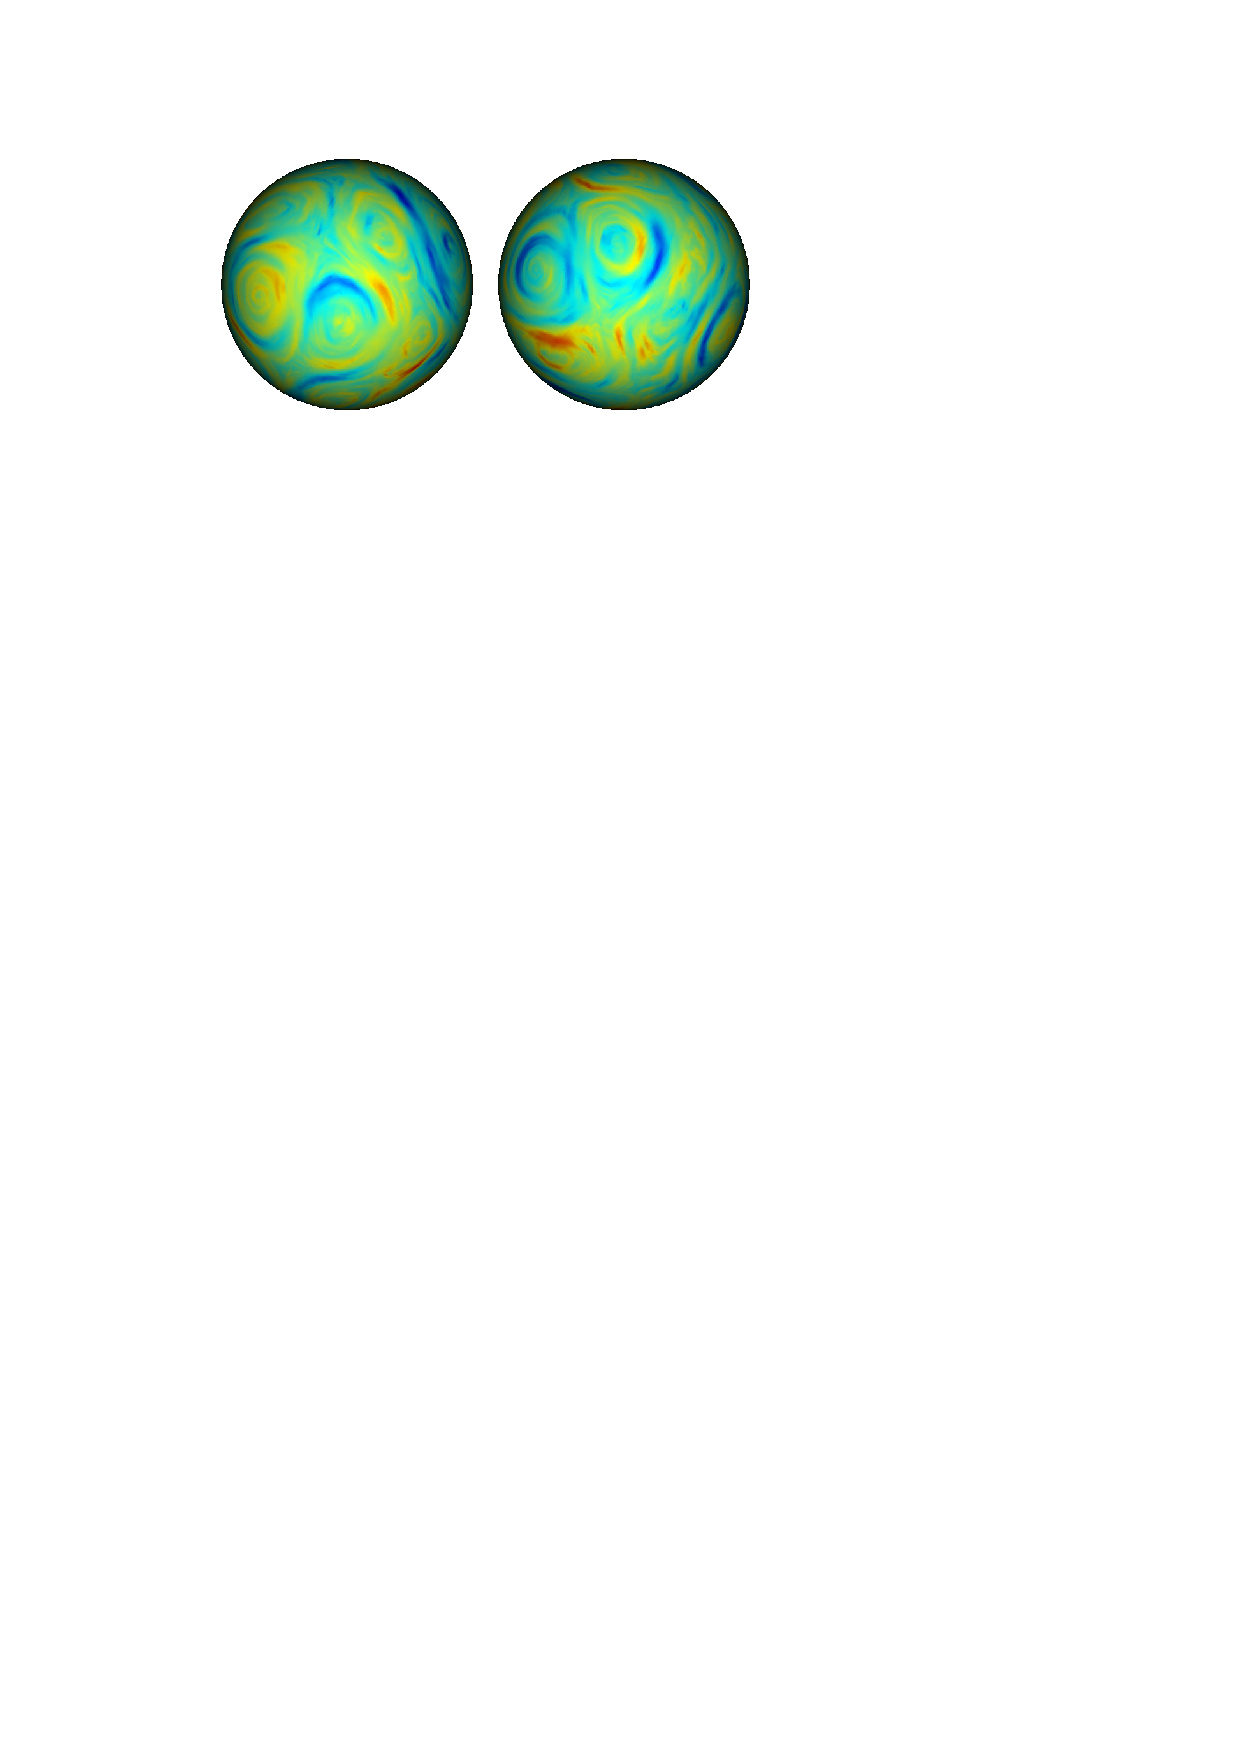
\includegraphics[width= 0.4\textwidth, angle= 0]{fig3}
}
\caption{An example of a spatial field on the sphere. \label{complex}}
\end{figure}

Another example of a complex domain are models on a sphere. Large-scale studies tend to use a projection of the into 2-dimensional space. However this results in a distortion of distances. Using the SPDE approach we can work directly on the sphere and do not need to project -- and distort the data. Figure \ref{sphere} shows an example of a spatial field on a sphere.

\begin{figure}[t]
  \centering
   \mbox{
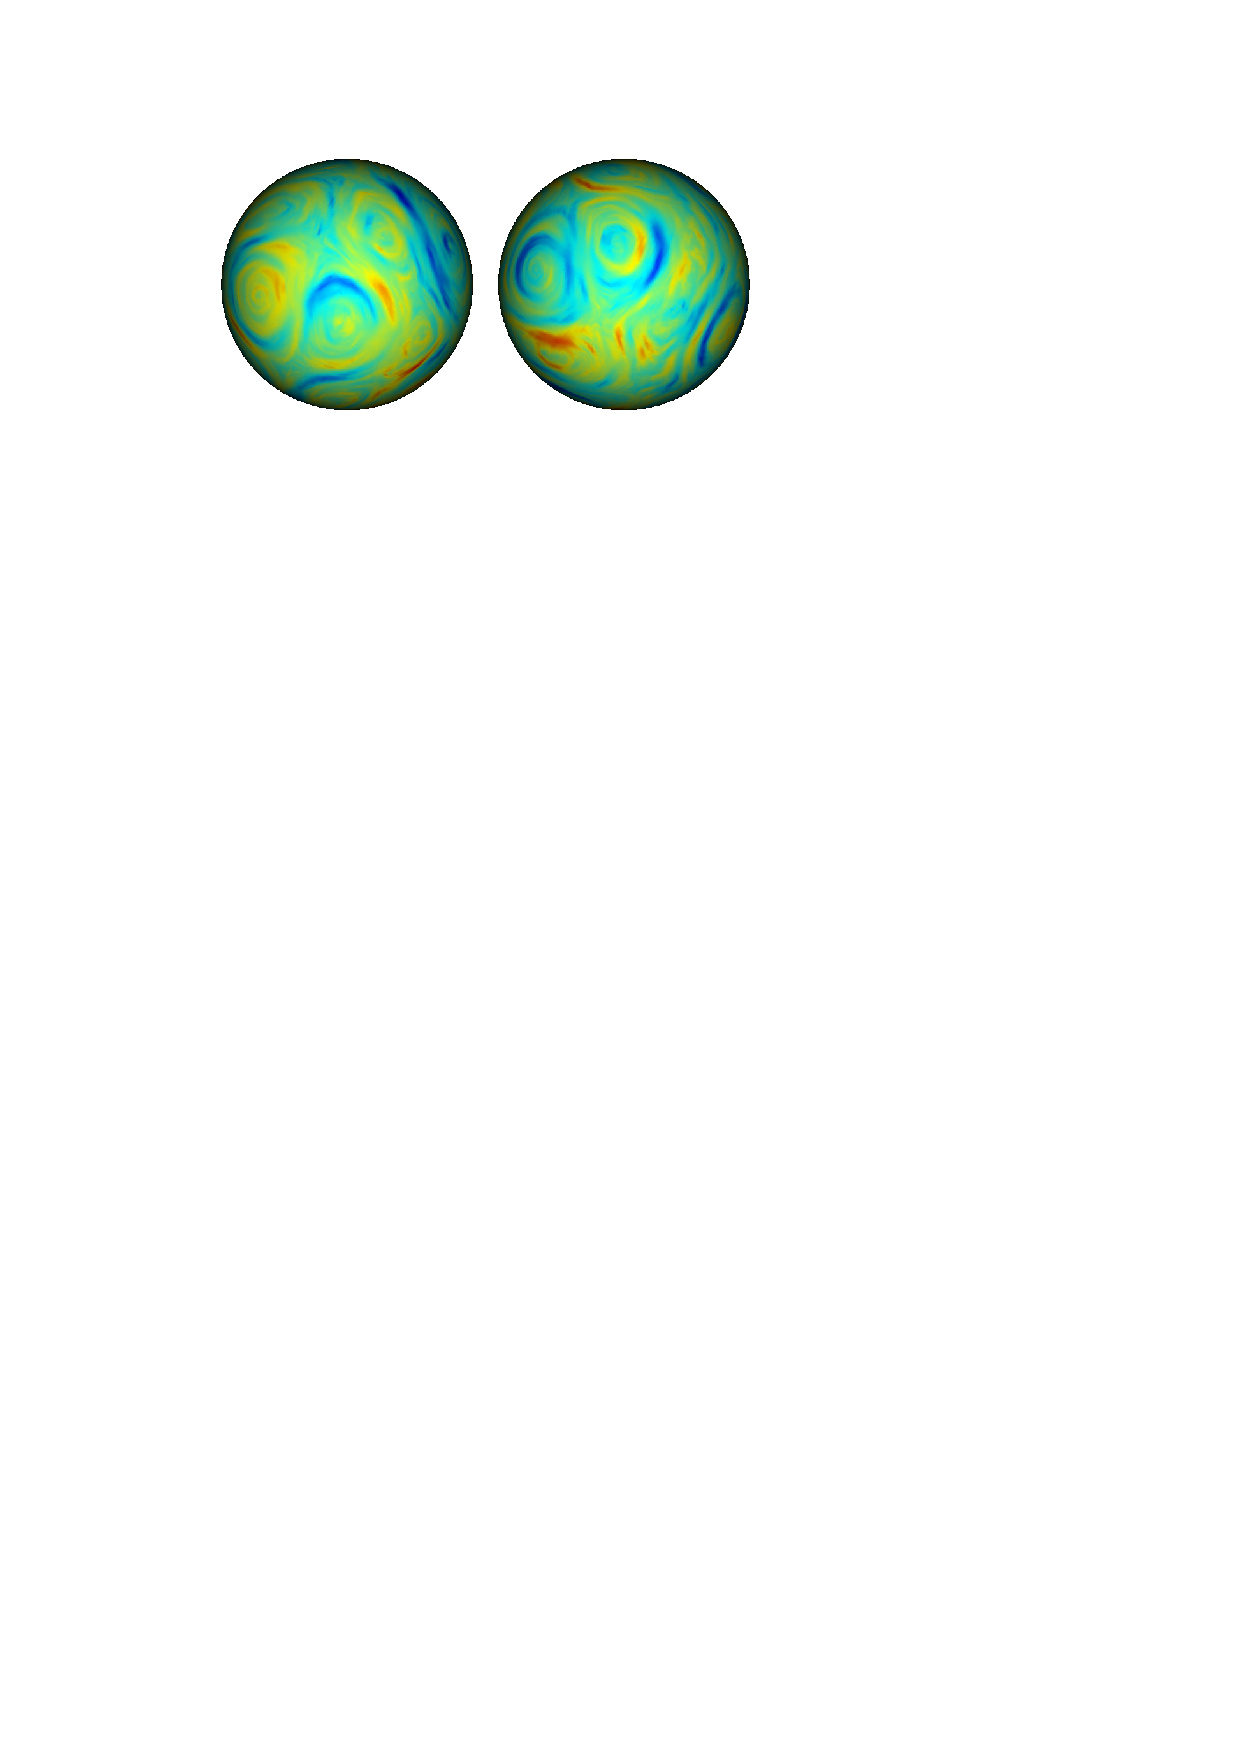
\includegraphics[width= 0.4\textwidth, angle= 0]{fig3}
}
\caption{An example of a spatial field on the sphere. \label{sphere}}
\end{figure}

Dealing with complex domains and data sets with ``holes" are an active area of research at the moment. The example in Section \ref{holedata} below considers a rather simple approach to the problem.

\subsubsection{Non-isotropic spatial fields}
The models we have discussed so far all assume that the spatially structured effect is stationary and isotropic. 
%implying that they assume that either the pattern itself is stationary or that all non-stationarity in a pattern can be explained by %the covariates in the model. However, in practice this assumption might not always hold. 

For example, consider the spatial pattern formed by the locations of plants. A prevailing wind direction might impact on seed dispersal since seeds are carried longer distances in that direction. This then results in elliptic dispersal kernels and  directionality/anisotropy in a the pattern of points. To account for this directionality, especially in the absence of covariate data on the local wind direction, a spatial field similar to the simulated random field shown in Figure \ref{non-stat} might be relevant.

% explain how non-stationarity may be implemented 

\begin{figure}[t]
  \centering
   \mbox{
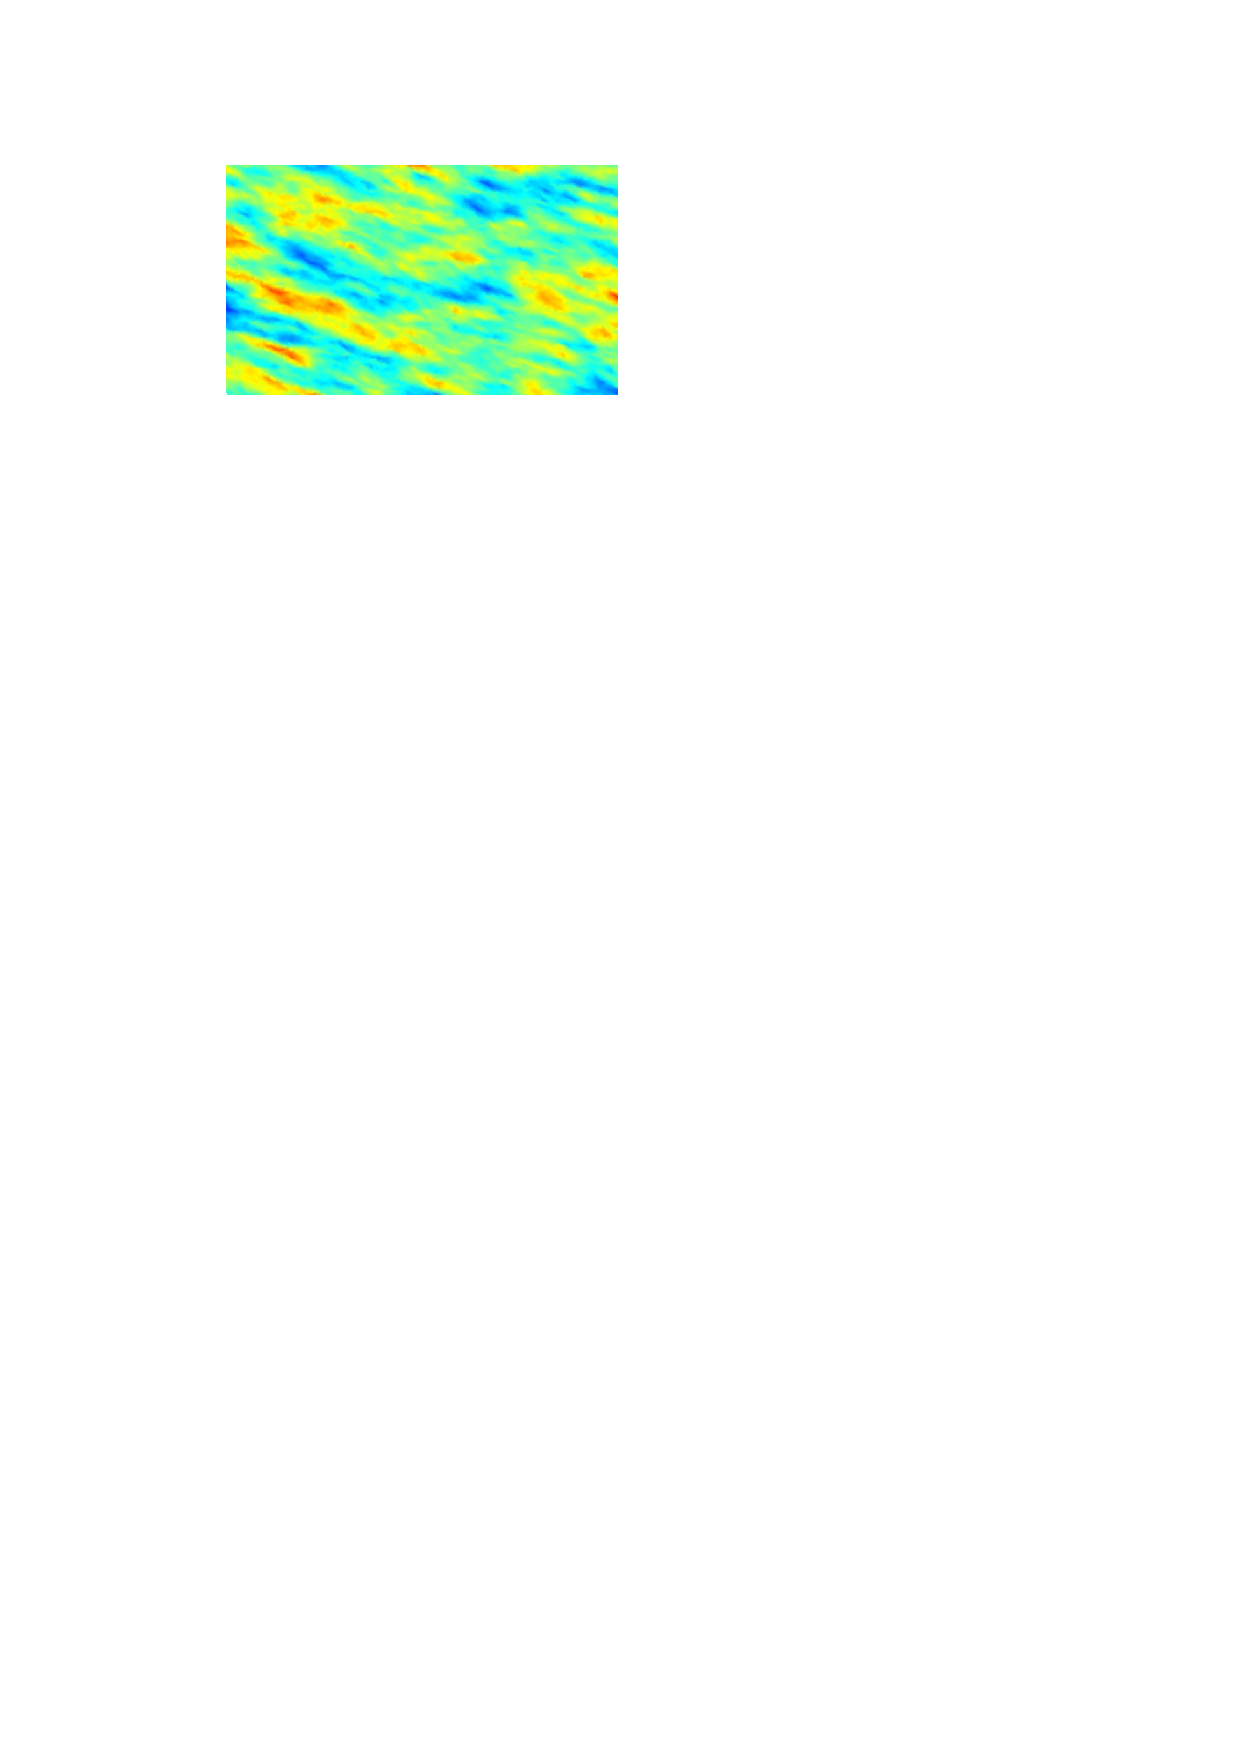
\includegraphics[width= 0.4\textwidth, angle= 0]{fig2}
}
\caption{An example of a non-stationary random field with clear anisotropy. \label{non-stat}}
\end{figure}

%flexible- can construct interesting correlation structures (ask Finn for examples of pictures)- simulate point patterns on these? %Work with Rikke??? 
%This is very much in development. 

\section{Examples}\label{spdeexamples}
As mentioned above this chapter aims at merely giving a taste of the SPDE methodology. For this reason we discuss -- very briefly  -- two small examples. Unlike in the previous chapters, we do not provide a thorough discussion of the examples themselves nor a detailed analysis of the respective data sets here. These examples  only serve as an illustration of the method.

\subsection{The koala data revisited}\label{koala2}
\subsubsection{Ignoring the marks -- a simple point pattern model }
Recall the koala dataset we discussed in detail in Chapter ??. In that chapter we presented a model of a spatial point pattern with two dependent marks. Apart from the fact that the model itself is rather complex we also had to deal with the fact that the observations have been collected in a polygon rather than in a rectangle. When using the gridding approach we had to embed the non-rectangular area in a larger rectangle and work with this- clearly, this is computationally expensive. When using the SPDE approach we can directly model on the polygonal observation area with no need of embedding and, as explained above, we do not need to approximate the points of the point pattern by binning them

The main focus of this book is to provide a general framework in which a wide variety of models may be fitted to spatial point patterns and analysed, in a convenient, efficient and accessible way. In particular, the framework enables us to consider realistically complex, \textbf{hierarchical models} in a Bayesian context. The key ingredient of the approach is the \textbf{INLA-methodology}, originally introduced in \cite{rueal:09} -- a new powerful tool that may be used to perform fast deterministic approximation for Bayesian inference. It may be applied to a general class of statistical models named \textbf{latent Gaussian models}.

This chapter aims to provide those readers who are mainly interested in applying INLA to spatial data with an understanding of the underlying structures of the models. We motivate the versatility of INLA and introduce and motivate latent Gaussian models in Sections 2.1 and 2.2, respectively.  

%Section 2.3 introduces in detail the spatially structures effects that INLA supports -- \textbf{Gauss Markov random fields}. 
% Maybe generally mention?

These become highly relevant when we return to the main focus of this book in Section 2.3, \textbf{log Gaussian Cox processes} and how INLA methodology may be applied to these.
%, followed by a general introduction to how to fit a log Gaussian Cox process model with INLA by implementing it in the \texttt{R-INLA} library.   
We would like to also provide those reader interested in themore  technical side of things with details on latent Gaussian models and on how INLA actually works --  i.e.\ how it approximates the likelihood. These details are presented in Sections 2.4 and  2.5 -- sections that might prove rather technical for some readers and may be skipped as the contents of the other chapters does not assume familiarity with these details. 
% indicated by *** mention ???

\section{INLA -- what is it all about?}
\subsection{Practical Bayesian modelling}
INLA may be used to fit many types of models within a Bayesian framework.  Due to their flexibility, Bayesian methods have become an increasingly popular tool in modern statistics that allows the fitting of models to complex data, often based on hierarchical models. In the context of this book we will only briefly introduce the reader to the general ideas behind Bayesian statistics along with the practical implications these have on the model fitting process. We refer the reader to the rich literature on Bayesian methodology for further reading (see Section \ref{ch:2_bibl}). 

An important characteristic of Bayesian methods is that Bayesian approaches assume the parameters in a model to be random and hence to follow some probability distribution, while frequentist methods assume that these parameters are fixed. Practically, this implies that existing knowledge on the specific distribution of each parameter (the so-called \textbf{prior}) may be used to inform modelling, which in turn implies that choosing the prior distribution forms an integral part of the modelling process. As a consequence, prior distributions have to be chosen carefully. In the models we consider here, careful prior choice is particularly important for the priors that are related to spatial structures in the models, and specifically the spatial smoothness of these structures. For this reason we discuss prior choice for the spatial structures in the model in detail in the next chapter (in Section ???), and provide practical advise on this.  

Once a prior has been chosen, the prior distribution is combined with data through the likelihood to form the \textbf{posterior distribution} of the parameters. In other words, data are used to inform the modelling process by updating existing knowledge as reflected in the prior(s) based on data. The posterior distribution is then used to draw inference and interpret the parameters. 

\subsection{Model fitting -- MCMC}
On the whole, the Bayesian approach provides intuitive and versatile modelling strategies. However, for many Bayesian models inference is not straight forward since the posterior is often not analytically tractable. Early Bayesian modelling was hence restricted to  a limited set of models for which the analytical form of the posterior can be derived.
This changed drastically with the advent of Markov chain Monte Carlo methods (MCMC)  in the 1980s. As flexible, simulation based techniques, MCMC methods may be implemented for basically any model and they have therefore been the standard tool for performing Bayesian inference in recent decades. 

However, due to their  simulation-based nature, MCMC-methods have severe shortcomings in the context of complex hierarchical models. An MCMC simulation has to be run for a long time to ensure that it is likely that it has converged, i.e.\ that the samples generated by the chain are samples from the relevant distribution. This implies that the approach is often not very computational efficient. As a consequence,  the time required to run MCMC simulations for some models may easily become too long for these to be practically relevant.  INLA is designed to avoid these long running times and hence makes fitting complex models more feasible. Computational efficiency has been the key motivation behind the development of INLA, and we will see below that this is particularly relevant for spatial models.

 \subsection{INLA to the rescue!}
While MCMC methods use stochastic simulations for estimation, integrated nested Laplace approximation (INLA)  is based on deterministic approximations where there are no convergence issues. INLA is a very accurate and computationally superior alternative to MCMC introduced in \cite{rueal:09} that may be used to fit a large class of models, \textbf{latent Gaussian models} (see Section \ref{LGM} below). 

Since INLA is fast, spatial modelling has become greatly facilitated and has also become more accessible to non-specialists. In addition, due to the fact that the fitting approach taken here is embedded in a large and general class of statistical models,  very general point process models may be considered. This allows us a lot more flexibility in the choice of model than previously -- and hence the models to capture interesting aspects of the data and consequently the system they are relevant for. More specifically, we can now fit models to spatial point patterns of high dimensionality, replicated point patterns, hierarchically marked point patterns etc.  In many cases, analysing these data sets with MCMC  would be very cumbersome and computationally prohibitive.

The INLA-methodology has been implemented in \texttt{C}, and the associated numerical calculations and algorithms are quite complex. These rely on an efficient implementation of numerical  procedures for Gaussian Markov random fields (GMRF) \citep{rueheld:05}, in particular the algorithms in the \texttt{C}-library \texttt{GMRFLib}.  However, most users do not need to worry about this, as the INLA-methodology has been made accessible through a user-friendly \texttt{R}-library, \texttt{R-INLA}, described and available for download at \texttt{www.r-inla.org}.  Specifying and fitting models using  \texttt{R-INLA} is just as easy as applying standard routines in \texttt{R},  for example fitting generalised linear models, and it also provides great flexibility with regard to the models that may be fitted. For the purpose of model evaluation, \texttt{R-INLA} provides summary statistics estimated from the posteriors, densities and model selection criteria that may be used to compare models, both in terms of model fit and prediction.  In summary, the INLA-methodology is easily accessible and provides a unified framework for Bayesian analysis of  a large class of statistical models, latent Gaussian models, comprising many familiar spatial and non-spatial models.


\section{A very general model structure -- latent Gaussian models}\label{LGM}

%\subsection{Which models can we fit?}\label{whichmodels}
In general, \textbf{latent Gaussian models} comprise many of the commonly used statistical models,  such as generalised linear or generalised additive models, mixed models, semiparametric regression, smoothing splines and state-space models, as well as spatial and spatio-temporal models. However, most readers might not be aware of this class of models explicitly but will soon realise that it comprises many models that they are very familiar with.

As a result,  the INLA-methodology has a very broad range of applications, for example in the analysis of survival models,  stochastic volatility and dynamic models, disease-mapping and ecological regression, as well as geostatistical modelling of large spatial datasets. 
It will become obvious below that log-Gaussian Cox processes, i.e.\ the spatial point process models we use in this book,  are a special case of this class of models, enabling us to use INLA to fit these. 

 %This is illustrated throughout this book as all case studies are accompanied by \texttt{R}-code.

In this section, we look at the structure of general latent Gaussian models in two different ways. We initially view them as a (rather general) regression model and then as a Bayesian hierarchical model.  We do this to provide the reader with an understanding of the structure of this model class and to make it easier to see which types of models may be fitted with INLA. Furthermore, this will make it clear why log Gaussian Cox processes form part of the class of latent Gaussian models and can hence be fitted with INLA.

\subsection{Generalising the generalised linear model}

The easiest way to understand a latent Gaussian model is to see it as a generalisation of a \textbf{generalised linear model}, which readers are likely to be familiar with. This is a model where the mean $\mu_i = E(\mm{y_i})$ of an observation $y_i$  in an $n$-dimensional observational vector $\mm{\mu}$ is assumed to depend -- via a link function $g(.)$ --  on a linear predictor of the following form

\begin{equation}	
\eta_i=g(\mu_i)=\beta_{0}+\sum_{\kappa} \beta_{\kappa} z_{i \kappa}+ u_i,\quad i=1,\ldots, n,\label{eq:lm}
\end{equation}
where $\beta_{0}$ is an intercept and the $\mm{\beta} = (\beta_1, \ldots, \beta_{\kappa})$ are parameters determining the \textbf{linear relationship} to some covariates $\mm{z} = (z_1, \ldots, z_{\kappa})$ and an error term $u_i$ following some appropriate error distribution. In the context of these generalised linear models the observations $\mm{y}$ are typically assumed to follow an exponential family distribution such as the normal, binomial or Poisson distribution and are assumed to be \textbf{independent observations}. These kinds of models can be easily fitted with standard software in a frequentist context as well as in a Bayesian context in a number of ways -- including with INLA. 

However, this is not what we will be concerned with here. We will deal with practical situations where  the relationship to the covariates may not be linear and --  in particular, since our data have been collected in space -- the observations may not be independent so that these simple models are of little use.  This implies that we require more general models. It is by providing models in a straight forward way, allowing us to drop the two assumptions of independent observations and linear relationships that latent Gaussian models generalise the simple model in Equation (\ref{eq:lm}). This is done by adding an additional term-- or  rather a sum of similar terms -- to the linear predictor in Equation (\ref{eq:lm}).

%The class of models that may be fitted with INLA, and hence the models discussed in this book all have a common general form.
%\footnote{It is also possible to fit an increasing number of models where the observations follow more general distributions %that are not part of the exponential family of distributions, for example the negative binomial. The \texttt{R-INLA} webpage %provides information on all distributions that are currently implemented.} and the population mean $\mu=E(\mm{y})$ is %assumed to be linked to a \textbf{structured additive predictor} through a link function $g(.)$.  

\subsection{Including structured effects -- structured additive regression models}\label{mod:lgm}
The additional terms that allow us to generalise the simple model we have considered so far  are referred to as \textbf{structured effects} -- hence the resulting models are often called ``structured additive regression models".  These additional terms account for non-linear relationships with covariates as well as for temporal or spatial dependence in the data and allow us to fit more complex models, i.e.\ models incorporating spatial, temporal or even spatio-temporal effects. 

Formally the linear predictor then looks as follows:
\begin{equation}	
\eta_i=g(\mu_i)=\beta_0+ \sum_{\kappa} \beta_{\kappa} z_{i \kappa}+\sum_{\gamma} f_{\gamma}(c_{i \gamma})+ u_i,\quad i=1,\ldots, n, \label{eq:lgm}
\end{equation}
where notation is exactly as above and $\sum_{\gamma} f_{\gamma}(c_{i \gamma})$ represents the ``structured effects". It is best to see these effects as \textbf{smooth functions}   (and hence the notation $f_{\gamma}(.)$). This can be a (non-linear) function of  a covariate, to account for non-linear relationship between the covariate and the outcome, generalising the model in Equation \ref{eq:lm} to a model structure that usually discussed in the context of generalised additive models. 

However, the smooth functions representing the structured effects can also be functions of time or space (or rather of an index across  time or space). This book mainly focuses  on \textbf{spatially structured effects} $f_s(\cdot)$ that account for spatial autocorrelation. We discuss how these functions are formally defined further below (Section?) and will that the temporally and spatially structured effects are defined in very similar ways. Some of the more complex data sets that we fit spatial models to are also dependent in time. We discuss \textbf{temporal dependence structures} in the context of these models. 
%(see Chapters...) 
Note that the error term, $\mm{u} = (u_1, \ldots, u_n)$, is often referred to as an \textbf{unstructured effect} as it is not a temporally or spatially smooth function but represents time- or space-independent error. 

So, what we have learned so far is that we can generalise the generalised linear model to construct model of non-independent observations by introducing  structured effects into the models. This has resulted in structured additive regression models. But we were setting out to define latent Gaussian models -- so the next thing we need to learn is what we mean by a \textit{latent} model and in particular by a latent \textit{Gaussian} model. 

%In many applications, the resulting latent Gaussian field has a sparse precision matrix (the inverse of the covariance matrix) %such that the latent field given $\mm{\theta}$ is a \textbf{Gaussian Markov random field} (GMRF). 
%\janine{Mixing up latent field and spatial field here. Sort this out. Also- introduce the two GMRF here? Or elsewhere in this %chapter?}


\subsection{Latent Gaussian models  as Bayesian hierarchical models}
Using INLA we can fit the models we have discussed in the previous section in a Bayesian context.  They may also be interpreted as Bayesian hierarchical models that consist of (at least) three levels  -- the observations, a latent field and hyperpriors. We will now look at these levels in detail and relate this to what we have discussed so far.

%as three levels in this model. Formally, this means that  \textbf{latent Gaussian models} are \textbf{hierarchical Bayesian %models} that consist of (at least) three different levels, the observations $\mm{y}$, the latent field ($\mm{\zeta}$) and %hyperparameters ($\mm{\theta}$). 

Recall that the we assume that we can account for dependence in the observations $\mm{y}$ by including structured effects in the model. In other words,  we assume that the observations are independent once we have included these effects. 

Together with the other parameters in the linear predictor  -- the intercept, the parameter reflecting dependence on covariates--  the structured effects accounting for temporal or spatial autocorrelation not explained by the covariates form the \textbf{latent field}.  And given this latent field we assume that the observations are independent. The elements in the latent field hence help explain existing dependence in the observations through the (structured) effects and by linking these to covariates.

Recall that we are in a Bayesian setting here and that all of these elements in the latent filed hence are random variables following a specific distribution. In a latent \textbf{Gaussian} model these are \textbf{Gaussian distributions} or \textbf{Gaussian priors}. The parameters of these Gaussian priors are referred to as hyperparameters, constituting the third level in our hierarchical model; these often have a \textbf{non-Gaussian distribution}. 

\vspace{0.3cm}
In summary this looks as follows:
\begin{itemize}
\item The {\bf observations} ($\mm{y}$) encode information about observed data, including design and collection issues. The  observations are assumed to be conditionally independent given the latent field and hyperparameters $\mm{\theta}$. 
\item The {\bf latent field} ($\mm{\zeta}$) accounts for dependence in the data based on observed and unobserved covariates. To account for spatial dependencies unexplained by covariates the latent field contains spatially structured effects. 
%that are modelled by a zero-mean \textbf{Gaussian Markov random field (GMRF)} with precision matrix $\mm{Q}(\mm{\theta})$, 

\item The {\bf hyperparameters} ($\mm{\theta}$) of the model are specified by
these may have a non-Gaussian distribution. For computational efficiency the dimension $m$ of the vector of hyperparameters $(\mm{\theta})$ should be small ($ m \leq 6$).
\end{itemize}


\subsection{INLA -- how it works}\label{INLAhow:heur}

The fact that we can see interpret latent Gaussian models as Bayesian hierarchical models as described above allows us to combine the three levels, and to express the posterior distribution of a latent Gaussian model as
\begin{equation*}
\pi(\mm{\zeta},\mm{\theta}\mid \mm{y})\propto \pi( \mm{\theta}) \pi(\mm{\zeta}\mid \mm{\theta}) \prod_{i}\pi(y_i\mid \zeta_i , \mm{\theta}).
\end{equation*}

The job of INLA is now to estimate the posterior marginals for all elements of the latent field as these inform us about the relationship between the response variable and covariates as well as about remaining spatial structures.  We also aim to estimate the marginals of the hyperparameters.  Both these estimations are done in INLA in a particular computationally efficient -- and hence fast --  way.  This is partly due to the assumption that the structured effects are chosen to be GMRFs (see Section 1.??), i.e.\ the structured effects live on a spatial lattice. The GMRF assumption implies that its precision matrix, i.e.\ the inverse of the variance-covariance matrix is sparse. This assumption is one of the essential ingredients of the approximation that INLA is based on.  It allows efficient computation of the marginals as this makes it possible to apply sparse matrix algorithms developed in computer science \citep{rueheld:05}. We will come back to the specific GMRFs implemented in INLA in Section \ref{spateff} below.

The other essential ingredient of INLA is the use of cleverly constructed Laplace approximations, which are particularly efficient approximation methods and allow us to estimate these marginals directly without using MCMC. This represents a huge gain in computational efficiency as well as accuracy. An understanding of the exact technical details as to how this is done is not necessary for an understanding of the models that we discuss in the case studies. These approximations are described in (the rather technical) Section \ref{INLAhow:tech} for those who are interested in these details.

\section{Log-Gaussian Cox processes as latent Gaussian models}

Log-Gaussian Cox processes, i.e.\ the type of spatial point process models discussed in this book are a special case of latent Gaussian models and can thus be analysed using the INLA-methodology. This section briefly discusses why this is the case and how fitting these may be approached in the context of the modelling structure described in equation (\ref{eq:lgm}), Section \ref{mod:lgm}.

\subsection{A hierarchical structure}
Recall that Cox processes, also referred to as  doubly-stochastic processes, are a flexible class of spatial point process
models in which the points are assumed to be independent given a \textbf{random intensity field} $\Lambda(\cdot)$, i.e.\ a random latent field and that given the latent field, the point pattern forms a Poisson process. 
%Due to the stochastic spatial trend represented by the latent field, such models are well suited for spatial point pattern data %with spatially observed and unobserved varying environmental conditions \citep{moelleral:07}.
As mentioned above, log-Gaussian Cox processes are a subclass of Cox-processes,  with random intensity
$$\log \Lambda(s)=\{{Z} (s)\},$$
where $\{{Z}(s): s\in \mathbb{R}^2 \}$ is a Gaussian random field.

The construction of log-Gaussian Cox processes mirrors the hierarchical structure of latent Gaussian models discussed above. If we consider these models in a Bayesian setting we have
\begin{itemize}
\item the observation, i.e.\ the  the points,
\item the latent field, i.e.\ the Gaussian random field and
\item the hyperparameters describing the Gaussian random field.
\end{itemize}

%Formally, the latent field $\Lambda(\cdot)$ is called an intensity measure and it is defined by
%$$\Lambda(B) = \int_B \lambda(x)dx$$
%in which $\lambda(\cdot)$ is called the intensity field of the Cox point process.


%In the following chapters we apply variations of  the linear predictor in \label{eq:lgm} to model spatial point patterns with different characteristics.


%\subsection{Log-Gaussian Cox processes and INLA }\label{mod:lgm}
%\texttt{JBI: We need to point out somewhere what distinguishes our approach from simply using glms "outside" INLA or similar %to model gridded data. Ecologists will ask this question... spatial structure not random, computational issues, joint models are %not straight forward...}

In practice, the primary data structure considered here is a spatial point pattern $\mm{x}=(\xi_1,
\ldots, \xi_n)$, regarded as a realisation of a spatial point
process $\mathbf{X}$. 
%For simplicity we consider only point processes
%observed in a window $W \in \mathbb{R}^2$ but our approach can be generalised to point
%patterns in higher dimensions. 

These point patterns as well as the associated models live in continuous space. Since the INLA methodology requires the latent field to be a Gaussian \textit{Markov} random field, the data are discretised using a spatial grid and the Gaussian random field is approximated by a Gaussian Markov random field. In the first few case studies presented in this book, we analyse spatial point patterns defined in rectangular observation regions.  In this case, the observation window is discretised into $N =
n_{row} \times n_{col}$ grid cells $\{ s_{ij}\}$, each with area
$|s_{ij}|$, where $i = 1, \ldots, n_{row}$ and $ j = 1, \ldots, n_{col}$. The
points in the pattern can then be described by $\{\xi_{ijk_{ij}}\}$
with $k_{ij} = 1, \ldots, y_{ij}$, where $y_{ij}$ denotes the \textbf{observed
number of points} in grid cell $s_{ij}$. For a given point pattern, the conditional distribution of the observations is the Poisson distribution, i.e.
\begin{equation}
    \label{poisson} y_{ij}| \eta_{ij} \sim \mbox{Po}(|s_{ij}| \exp(\eta_{ij})),
\end{equation}
where $ \eta_{ij} = {Z}(s_{ij})$.
Extensions to non-rectangular observation regions are straightforward and will be addressed, for example, in Chapter 7.
Note that we will see in Chapter 10 that the grid does not have to be regular and that a more flexible discrete representation may be used instead. 

An important aim of this book is to illustrate how we can flexibly analyse spatial point patterns of increasing complexity, all within the same framework. This flexibility stems from the fact that the model may be expressed based on a predictor similar to that defined in Equation (\ref{eq:lgm}). We only have to our change notation slightly to make the underlying two-dimensional grid structure explicit. For a grid cell $s_{ij}$ this yields

\begin{equation}
\eta_{ij}=\beta_0+\mm{z_{ij}}'\mm{\beta}+\sum_{\gamma} f_{\gamma}(c_{ij \gamma})+f_s(s_{ij})+u_{ij},\quad i=1,\ldots, n_{row}, j=1,\ldots , n_{col}. \label{eq:linpred}
\end{equation}

In analogy to (\ref{eq:lgm}), this model contains linear and smooth effects of covariates and along with spatially structured and unstructured terms. The estimated spatially structured effect may often be used to reveal remaining spatial structure that cannot be explained by the covariates in the model, while the unstructured effects may be interpreted as a spatial residual.

In summary, the latent Gaussian structure of log-Gaussian Cox processes allows us to use INLA to fit these models which speeds up the estimation drastically and hence allows us to practically fit log-Gaussian Cox process models that are far more complex than many of the models considered before.This model structure can easily be extended to incorporate additional terms that allow the construction of more complex models accounting for the structures in a specific point pattern data set. For example, the model in (\ref{eq:linpred}) is extended to include temporally varying random effects for replicated point patterns in Chapter 7 or terms describing interaction between species (Chapter 5). Another feature of the INLA-methodology is that it allows us to specify \textbf{joint models}, in which two or more observational models are analysed together. This allows us to impose terms that are shared among the different observational models, for example joint spatial effects. The joint formulation is especially relevant in analysing marked point patterns (Chapter 7-9), but is also useful in the context of replicated patterns (Chapter ???) as well as models with measurement error in the covariates (Chapter ??? - we don't have this in any chapter just now).


\section{Outlook}

Chapter on details of INLA ad SPDE approximation can be skipped if technical details not of interest (Sigrunn)

Chapter on mesh construction (Finn!)
